\documentclass[journal]{IEEEtran}

\usepackage[utf8]{inputenc}
\usepackage[T1]{fontenc}
\usepackage{amsmath,amssymb}
\usepackage{booktabs}
\usepackage{array}
\usepackage{multirow}
\usepackage{makecell}
\usepackage{url}
\usepackage{xcolor}
\usepackage{graphicx}
\usepackage[hidelinks]{hyperref}
\usepackage{tikz}
\usepackage{pgfplots}
\pgfplotsset{compat=1.16}
\usetikzlibrary{arrows.meta,positioning,calc,shapes.geometric,fit,backgrounds,patterns}

\tolerance=4000
\emergencystretch=3em
\hbadness=2000
\vbadness=2000
\renewcommand{\arraystretch}{1.08}
\setlength{\tabcolsep}{4pt}

\newcommand{\micro}{$\mu$}
\newcommand{\code}[1]{\texttt{\small #1}}
\newcommand{\true}{\textsc{T}}
\newcommand{\false}{\textsc{F}}
\hyphenation{op-tical net-works semi-conduc-tor co-simu-la-tion
ndn-SIM nu-mer-o-logy gNo-deB sub-car-rier}

\tikzset{
  box/.style={draw, rounded corners=2pt, align=center, font=\small,
              minimum height=7mm, inner sep=3pt},
  sim/.style={draw, fill=blue!8, rounded corners=2pt, align=center,
              font=\small, minimum height=8mm, inner sep=3pt},
  net/.style={draw, fill=orange!12, rounded corners=2pt, align=center,
              font=\small, minimum height=8mm, inner sep=3pt},
  data/.style={draw, fill=green!10, rounded corners=2pt, align=center,
               font=\small, minimum height=7mm, inner sep=3pt},
  warn/.style={draw, fill=red!8, rounded corners=2pt, align=center,
               font=\small, minimum height=7mm, inner sep=3pt},
  link/.style={-Stealth, thick},
  dlink/.style={-Stealth, dashed, thick}
}

\begin{document}

\title{Cross-Layer NFV and Named Data Networking Integration for 5G NR-V2X Edge Services}
\author{
\IEEEauthorblockN{Rajesh Bhusal, Amit Aacharya, Prakash Mahato, Arun C. Bhusal, Babu R. Dawadi*\thanks{*Corresponding Author: Babu R. Dawadi (baburd@ioe.edu.np)}}\\
\IEEEauthorblockA{
\textit{Tribhuvan University Institute of Engineering, Pulchowk Campus, 44700 Lalitpur, Nepal}} \\
\and
\IEEEauthorblockN{Pietro Manzoni}\\
\IEEEauthorblockA{
\textit{Department of Computer Engineering, Universitat Politècnica de València, 46022 Valencia, Spain}
}}
\maketitle

\begin{abstract}
Vehicular applications increasingly request information based on location, events, and data semantics rather than from fixed remote hosts. Named Data Networking (NDN) is attractive for such workloads because names, Pending Interest Table state and Content Store reuse are first-class network objects. The key practical question is whether these information-centric properties remain measurable when the data plane is embedded in a 5G NR-V2X edge scenario. This paper presents an integration-oriented, reproducible co-simulation study that couples SUMO mobility, OMNeT++/Veins Network Functions Virtualization (NFV) and Multi-access Edge Computing (MEC) orchestration and application logic, and ns-3/ndnSIM networking for edge filtering, traffic-light preemption, TTC-based collision avoidance and topology-aware accident notification.

The study compares a documented IP/UDP baseline with NDN over UDP/IP
across NR numerologies $\mu\in\{1,2,3\}$ on a 200\,s urban trace. Results show a consistent trade-off. IP has the lower V2I
median RTT, while NDN adds measurable information-centric behavior:
55.93--57.02\,\% Content Store hit rate, 99.67--99.97\,\% Interest
satisfaction, no NACKs observed across the evaluated NDN runs. NDN at $\mu=3$
is the only NDN configuration that meets the 10\,ms median-latency reference in this scenario; both stacks satisfy the broader
TS\,22.185 100\,ms V2X tier. The NFV telemetry confirms active Road Side Unit (RSU) edge
service management, with 23--25 active RSU instances, scale-out/scale-in
events and recorded control overhead. The results illustrate the interaction between information-centric forwarding, edge orchestration, and NR-V2X numerology in shaping latency, cache reuse, and safety-application behavior in mobility-driven vehicular environments.
\end{abstract}

\begin{IEEEkeywords}
Vehicle-to-Everything, Network Functions Virtualization, Named Data Networking, 5G NR, NR-V2X, MEC, ndnSIM, ns-3, SUMO, OMNeT++, Veins, caching, URLLC, co-simulation.
\end{IEEEkeywords}

% =============================================================================
\section{Introduction}
\label{sec:intro}
% =============================================================================

\IEEEPARstart{V}{ehicular} safety and traffic-management applications often consume information by event and location: the current state of an intersection, the presence of a nearby accident, or the position of a vehicle in a zone. IP/UDP can transport these messages, but it leaves content naming, request aggregation and cacheable responses to the application. Under high mobility, however, maintaining low-latency, location-aware data delivery becomes increasingly difficult in such environments because communication endpoints, edge attachment points, and application demand may all change simultaneously. NDN exposes these properties in the network by forwarding Interests for named data and returning Data from any producer or Content Store (CS) that can satisfy the request \cite{ref:ndn-overview,ref:nfd}.

This paper quantifies the systems-level performance when information-centric forwarding is embedded within an NR-V2X/MEC/NFV co-simulation. Earlier vehicular NDN studies often focus on VANET-level name routing or abstract the cellular layer \cite{ref:vndn,ref:ndn-v2x-survey}. Conversely, 5G NR-V2X studies often evaluate IP traffic over cellular or sidelink models without exposing NDN state such as PIT aggregation, CS hits and Interest satisfaction \cite{ref:cv2x-rel16,ref:ns3-nr}. This paper evaluates how NDN forwarding behavior, NFV-driven edge orchestration, and NR-V2X configuration interact within a unified vehicular communication pipeline.

Vehicular environments are central to this study because mobility continuously reshapes communication paths, edge attachment points, and content demand locality. Unlike static MEC environments, V2X deployments must sustain low-latency data delivery while vehicles traverse RSU coverage regions, generate transient safety-critical events, and repeatedly request geographically scoped information. The proposed framework therefore evaluates not only packet delivery performance, but also how caching behavior, orchestration activity, and edge-service placement respond to mobility-driven workload changes.

\subsection{Contributions}

This paper makes four concrete contributions:
\begin{enumerate}
  \item \textbf{A cross-layer vehicular edge-networking framework.} SUMO provides mobility \cite{ref:sumo}, OMNeT++/Veins drives NFV/MEC management and application events \cite{ref:veins}, and ns-3/ndnSIM collects IP and NDN network metrics \cite{ref:ndnsim,ref:ns3-nr}. The framework integrates SUMO, OMNeT++/Veins, and ns-3/ndnSIM through lock-step event synchronization, enabling simultaneous measurement across the mobility, orchestration, and networking layers.

  \item \textbf{A controlled IP/UDP and NDN-over-5G comparison.} The IP and NDN grids both contain seeds 1--3 for $\mu=1,2,3$. This permits numerology-level cross-seed variability analysis for both stacks while keeping the comparison scoped to one scenario, one vehicle density and one gNB.

  \item \textbf{A measured account of topology-aware proactive caching.} We demonstrate how an NFV Control Plane can construct an upstream road-topology graph to proactively pre-warm NDN caches at the 5G edge. While NDN adds transmission overhead, the proposed orchestration approach yields consistent Content Store hit rates exceeding 55\,\%, near-perfect Interest satisfaction, with no NACKs observed across all swept numerologies.

  \item \textbf{A measured NFV/MEC orchestration context.} OMNeT++ NFV telemetry captures active RSU edge-function scaling (23 to 25 active instances), scale-out/scale-in events, and application-layer service-flow telemetry (accident reporting and emergency traffic preemption). The orchestration layer is evaluated as the elastic service substrate supporting the vehicular data-plane experiments.
\end{enumerate}

The rest of the paper is organized as follows. Section~\ref{sec:related} reviews relevant V2X, NDN and MEC work. Section~\ref{sec:system} describes the architecture. Section~\ref{sec:method} defines the dataset, metrics, and evidence scope. Section \ref{sec:nfv} presents NFV orchestration results. Sections~\ref{sec:ip} and \ref{sec:ndn} present IP and NDN results, respectively. Section~\ref{sec:discussion} compares stacks and interprets the trade-offs. Section~\ref{sec:limits} states limitations and Section~\ref{sec:conclusion} concludes.

% =============================================================================
\section{Background and Related Work}
\label{sec:related}
% =============================================================================

\subsection{5G NR-V2X and Latency Tiers}

3GPP defines enhanced V2X service requirements in TS\,22.186 and TS\,22.185, and studies advanced/automated driving support in TR\,22.886 \cite{ref:v2x-3gpp22186,ref:v2x-3gpp22185,ref:v2x-3gpp22886}. NR uses flexible numerology, where subcarrier spacing is $15\cdot2^\mu$\,kHz and slot duration is approximately $1/2^\mu$\,ms \cite{ref:nr-phy}. The numerologies studied here are $\mu=1,2,3$, corresponding to 30, 60 and 120\,kHz subcarrier spacing and 0.5, 0.25 and 0.125\,ms slots. The simulator configuration uses a 3.5\,GHz FR1 carrier, 100\,MHz bandwidth, TDMA round-robin scheduling, and a 3GPP UMa-LoS channel model based on TR\,38.901 \cite{ref:nr-channel}.

We report three latency tiers. The evaluated 10 ms median-latency reference derived from TS 22.186 P50$\le10$\,ms V2I tier. We use this as a strict low-latency reference point in the context of 5G URLLC design constraints \cite{ref:5g-urllc}. The TR\,22.886 advanced/automated driving tier is tracked at 25\,ms, and the broader TS\,22.185 V2X tier at 100\,ms. These flags are not full service-level certification; they are dataset-level checks over the post-warmup latency distribution used for latency analysis.

\subsection{Named Data Networking in Vehicular Systems}

NDN changes the communication primitive from endpoint addressing to name-based retrieval \cite{ref:ndn-overview}. In vehicular systems this maps naturally to traffic-state, hazard and zone-scoped information \cite{ref:vndn,ref:ndn-v2x-survey}. NFD forwarding strategies, PIT state, producer mobility, and caching policies are central to whether this model remains stable under mobility \cite{ref:ndn-mobility,ref:ndn-cache-survey}. ndnSIM provides the simulation environment for these NDN mechanisms \cite{ref:ndnsim}.

The NDN literature often emphasizes caching and name-based dissemination, whereas cellular V2X studies emphasize radio scheduling and sidelink resource allocation. The proposed framework evaluates these mechanisms within a reproducible simulation framework: NDN packets are carried over UDP/IPv4 through the simulated V2I access path, and the NDN forwarder state is measured alongside IP baseline metrics.

\subsection{Study Questions}

The study is organized around four verifiable questions:
\begin{enumerate}
  \item \emph{Latency cost:} how much V2I latency does the NDN forwarding pipeline add relative to the IP/UDP baseline under the same 200\,s urban trace and NR numerology sweep?
  \item \emph{Caching value:} does the NDN stack produce a measurable Content Store hit rate under a repeated vehicular query workload, and is that behavior stable across numerology and seed?
  \item \emph{Safety-workload coverage:} do the four study safety use cases execute through the co-simulation and expose internal activation counters that can be inspected independently of the aggregate latency results?
  \item \emph{Scope boundary:} under which NR-V2X configurations does NDN provide measurable benefits relative to IP, and what experimental parameters are required for broader generalization?
\end{enumerate}

\subsection{Positioning Against Existing Studies}

The closest prior work falls into three families. First, vehicular NDN and VANET-over-NDN studies motivate name-based dissemination, in-network caching and forwarding strategies for mobile producers and consumers \cite{ref:vndn,ref:ndn-v2x-survey,ref:ndn-mobility}. These works are important because they establish why host identifiers are a poor fit for many vehicular information flows. However, they often emphasize the network-layer naming problem without reporting the exact radio-stack conditions under which the latency distribution is measured.

Second, NR-V2X simulation studies evaluate numerology, scheduling and radio/channel behavior \cite{ref:cv2x-rel16,ref:ns3-nr}. These studies are essential for understanding why a 30\,kHz and a 120\,kHz numerology do not produce the same latency tail. Their limitation for the present question is the opposite of the NDN literature: the communication service is usually IP-like or bearer-oriented, so ICN-specific state such as CS hits, PIT timeouts and Interest satisfaction is not observable.

Third, NFV/MEC-oriented V2X work studies how virtualized edge placement shortens the application path, supports local control decisions, and allows infrastructure to scale with demand \cite{ref:mec-etsi,ref:mec-v2x-placement}. Our study follows that placement logic by locating the producer/service side at MEC and by using OMNeT++ as the NFV management/application plane, but it adds a protocol comparison: IP/UDP carries host-addressed requests, whereas NDN carries named Interests and Data over the same access-side simulation context.

The evaluation bridges these three families by integrating named-data semantics, cellular numerology, and MEC safety workloads within a single evaluation framework.

\subsection{MEC and Safety Applications}

MEC is a natural placement for V2X aggregation, filtering and local decision support \cite{ref:mec-etsi,ref:mec-v2x-placement}. In this study, MEC is paired with an NFV management plane: OMNeT++/Veins maintains the application and orchestration state, while ns-3/ndnSIM evaluates packet delivery and forwarding. The use cases are intentionally simplified but safety-relevant: edge filtering, traffic-light preemption, TTC-based collision avoidance, and accident notification. TTC follows the standard relative-position/closing-rate idea used in traffic safety analysis \cite{ref:ttc}; vehicle motion is provided by SUMO using microscopic traffic models including IDM and MOBIL \cite{ref:idm,ref:mobil}. The simulator counters should be read as algorithm-execution and message-delivery counters, not as proof of real-world collision avoidance.

\subsection{NFV Management Plane}

The NFV part of this study is implemented on the OMNeT++ side, not as a cosmetic label on the NDN results. It manages RSU/edge infrastructure as virtualized service instances: static RSUs provide a backbone at intersections, while dynamic in-fill RSUs can be scaled out or in as the topology and density logic requires. The corresponding metrics comprise active RSUs, scale-out/scale-in events, lifecycle cost estimates, control-overhead estimates and service-flow counters for emergency/accident handling. This telemetry verifies that the system operates as an NFV-orchestrated V2X architecture rather than a standalone NDN data plane.

The management-plane model is intentionally separated from the packet forwarding model. OMNeT++ has direct access to road-segment and junction semantics through Veins/SUMO, so it decides where an RSU-like edge function should exist. ns-3, in contrast, is used for packet timing, NR access behavior, IP forwarding and NDN forwarding counters. In this manuscript, ``NFV'' therefore refers to edge-function lifecycle and orchestration logic: active RSU instances, scale-out/scale-in decisions, and service-flow counters. The data plane is evaluated after that managed edge-service layout has been supplied, which keeps application-level elasticity separate from physical-layer channel dynamics. The following section describes the architectural framework developed to evaluate these three components in a unified co-simulation setting.

% =============================================================================
\section{System Architecture}
\label{sec:system}
% =============================================================================

\subsection{Simulator Coupling}

Fig.~\ref{fig:pipeline} shows the evidence pipeline. OMNeT++/Veins and SUMO provide the traffic scenario, NFV management plane and application events. ns-3 runs the network path and exports trace files. The framework automatically extracts and aggregates stack-specific traces into structured performance metrics, while the OMNeT++ NFV metrics are preserved as time-series telemetry logs.

\begin{figure}[!t]\centering
\resizebox{0.96\columnwidth}{!}{%
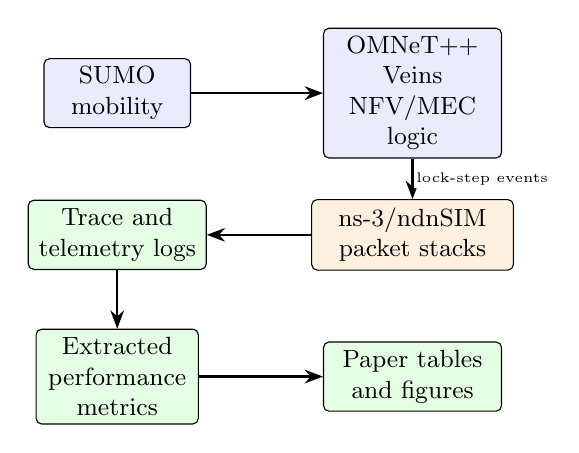
\begin{tikzpicture}[x=1cm,y=1cm,every node/.append style={font=\scriptsize}]
  \node[sim, text width=1.65cm] (sumo) at (0,1.8) {SUMO\\mobility};
  \node[sim, text width=2.05cm] (omnet) at (3.75,1.8) {OMNeT++\\Veins NFV/MEC\\logic};
  \node[net, text width=2.35cm] (ns3) at (3.75,0) {ns-3/ndnSIM\\packet stacks};
  \node[data, text width=2.05cm] (traces) at (0,0) {Trace and\\telemetry logs};
  \node[data, text width=1.85cm] (json) at (0,-1.8) {Extracted\\performance metrics};
  \node[data, text width=2.05cm] (paper) at (3.75,-1.8) {Paper tables\\and figures};
  \draw[link] (sumo) -- (omnet);
  \draw[link] (omnet) -- node[right,font=\tiny,fill=white,inner sep=1pt]{lock-step events} (ns3);
  \draw[link] (ns3) -- (traces);
  \draw[link] (traces) -- (json);
  \draw[link] (json) -- (paper);
\end{tikzpicture}
}
\caption{Reproducibility pipeline. Automated extraction of per-run metrics ensures traceability from simulator output to reported values.}
\label{fig:pipeline}
\end{figure}

\subsection{Communication Paths}

Fig.~\ref{fig:scope} distinguishes what is measured as a cellular V2I path from what is deliberately emulated. For V2I, vehicles and RSUs use the ns-3 NR/EPC path toward a MEC node. For NDN, the NDN face is carried over UDP/IPv4 so NDN Interests and Data traverse the simulated IP route. For V2V, this study uses point-to-point links with fixed 100\,Mb/s and 1\,ms parameters. This V2V path supports protocol and content-routing checks only; it is not used as a PC5 Mode 1/2 radio performance model.

\begin{figure}[!t]\centering
\resizebox{0.96\columnwidth}{!}{%
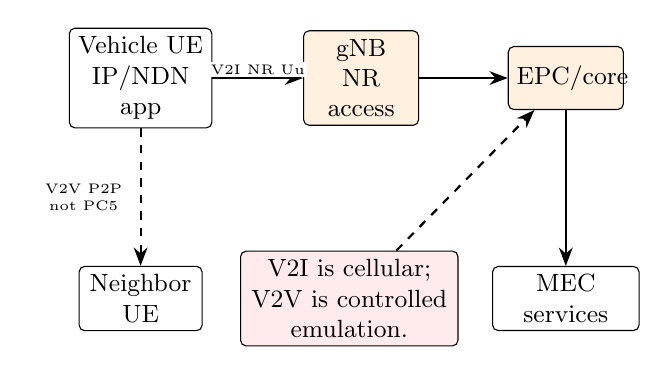
\begin{tikzpicture}[x=1cm,y=1cm,every node/.append style={font=\scriptsize}]
  \node[box, text width=1.6cm] (veh) at (0,1.05) {Vehicle UE\\IP/NDN app};
  \node[net, text width=1.25cm] (gnb) at (2.8,1.05) {gNB\\NR access};
  \node[net, text width=1.25cm] (epc) at (5.4,1.05) {EPC/core};
  \node[box, text width=1.65cm] (mec) at (5.4,-1.75) {MEC\\services};
  \draw[link] (veh) -- node[above,font=\tiny,fill=white,inner sep=1pt]{V2I NR Uu} (gnb);
  \draw[link] (gnb) -- (epc);
  \draw[link] (epc) -- (mec);

  \node[box, text width=1.35cm] (veh2) at (0,-1.75) {Neighbor UE};
  \draw[dlink] (veh) -- node[left,font=\tiny,align=center,text width=1.35cm,fill=white,inner sep=1pt]{V2V P2P\\not PC5} (veh2);

  \node[warn, text width=2.55cm] (note) at (2.65,-1.75)
  {V2I is cellular; V2V is controlled emulation.};
  \draw[dlink] (note) -- (epc);
\end{tikzpicture}
}
\caption{Measured communication scope. The V2I path is the cellular access path used for the main latency claims. V2V uses deterministic point-to-point emulation because no integration-ready PC5 sidelink module was available; V2V is excluded from PC5 radio claims.}
\label{fig:scope}
\end{figure}

\subsection{Protocol Stack Mapping}

The two evaluated stacks share the same mobility and application event sources but differ in their network-facing abstractions. The IP baseline uses UDP request--reply flows toward the MEC. The NDN stack maps application requests to named Interests and returns Data over NDN faces carried by UDP/IPv4 sockets. This design is intentional: it lets the NDN forwarder exercise PIT, FIB and CS logic while still traversing the same V2I cellular access path used by the baseline. Fig.~\ref{fig:stackmap} summarizes the mapping.

\begin{figure}[!t]\centering
\resizebox{0.90\columnwidth}{!}{%
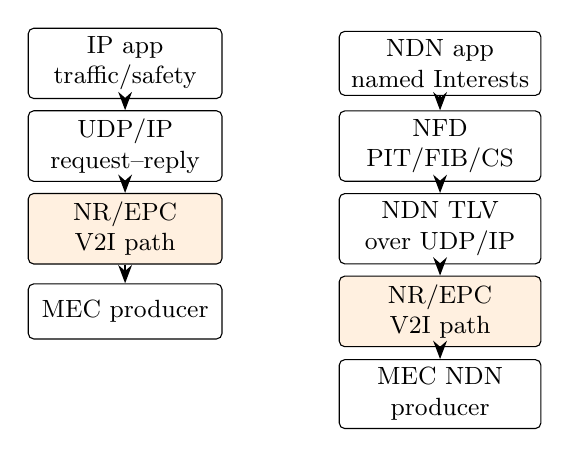
\begin{tikzpicture}[x=1cm,y=1cm,every node/.append style={font=\scriptsize}]
  \node[box, text width=2.25cm] (ipapp) at (0,0) {IP app\\traffic/safety};
  \node[box, text width=2.25cm] (udp) at (0,-1.05) {UDP/IP\\request--reply};
  \node[net, text width=2.25cm] (nr1) at (0,-2.10) {NR/EPC\\V2I path};
  \node[box, text width=2.25cm] (mec1) at (0,-3.15) {MEC producer};

  \node[box, text width=2.35cm] (ndnapp) at (4.0,0) {NDN app\\named Interests};
  \node[box, text width=2.35cm] (nfd) at (4.0,-1.05) {NFD\\PIT/FIB/CS};
  \node[box, text width=2.35cm] (udp2) at (4.0,-2.10) {NDN TLV\\over UDP/IP};
  \node[net, text width=2.35cm] (nr2) at (4.0,-3.15) {NR/EPC\\V2I path};
  \node[box, text width=2.35cm] (mec2) at (4.0,-4.20) {MEC NDN\\producer};

  \draw[link] (ipapp) -- (udp);
  \draw[link] (udp) -- (nr1);
  \draw[link] (nr1) -- (mec1);
  \draw[link] (ndnapp) -- (nfd);
  \draw[link] (nfd) -- (udp2);
  \draw[link] (udp2) -- (nr2);
  \draw[link] (nr2) -- (mec2);
\end{tikzpicture}
}
\caption{Protocol mapping used for comparison. IP exposes UDP RTT; NDN adds name-based forwarding state and uses ndnSIM FullDelay for latency.}
\label{fig:stackmap}
\end{figure}

\subsection{Naming and Data Model}

NDN names in this study encode the type and scope of the requested information: prefixes such as \code{/traffic/info} and \code{/traffic/count} represent repeated, MEC- or RSU-sourced traffic-state queries; \code{/safety/accident} identifies RSU-originated notification objects; and \code{/position} carries short-lived vehicle-state data. Names are intentionally conservative, maintaining per-vehicle and per-service identity to allow unambiguous tracing of cache hits to their producer sources.

\subsection{Timing and Synchronisation}

The co-simulation advances through lock-step application updates rather than a loose offline trace replay. SUMO maintains vehicle mobility; OMNeT++/Veins emits application-level events and safety use-case triggers; OMNeT++/Veins also records NFV management events, including active RSU instances and RSU lifecycle operations; ns-3/ndnSIM evaluates network delivery and exports the traces. The 50\,ms application update granularity is visible in the safety counters and in the deterministic V2V behavior. V2I packet timing, however, is governed by the NR configuration, UDP/NDN processing, and the run-specific scheduler state. This separation is why we report application and NFV counters separately from V2I latency percentiles.

\subsection{NFV-Orchestrated RSU Lifecycle}

Fig.~\ref{fig:nfvplane} separates the NFV management plane from the network data plane. The OMNeT++ control layer observes topology and application state, decides whether edge RSU functions should exist, and records the resulting lifecycle metrics. The ns-3/ndnSIM side then carries the IP or NDN traffic generated by those services. In NFV terms, the RSU application is treated as an edge VNF: it can host filtering, traffic-light control and notification logic, while the MEC/core side acts as the coordination point for broader safety services.

\begin{figure}[!t]\centering
\resizebox{\columnwidth}{!}{%
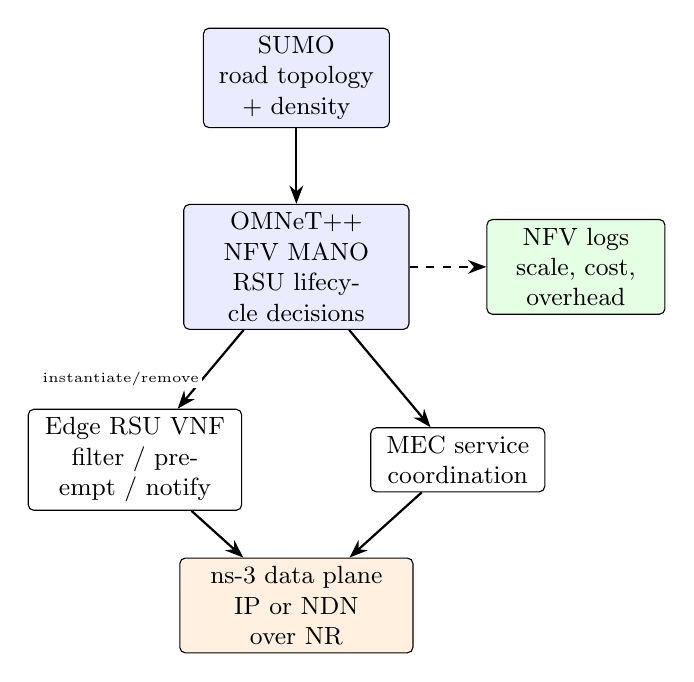
\begin{tikzpicture}[x=1cm,y=1cm]
  \node[sim, text width=2.15cm] (sumo) at (2.7,3.35) {SUMO\\road topology + density};
  \node[sim, text width=2.65cm] (mano) at (2.7,0.95) {OMNeT++ NFV MANO\\RSU lifecycle decisions};
  \node[box, text width=2.5cm] (rsu) at (0.65,-1.5) {Edge RSU VNF\\filter / preempt / notify};
  \node[box, text width=2.0cm] (mec) at (4.75,-1.5) {MEC service\\coordination};
  \node[net, text width=2.75cm] (data) at (2.7,-3.35) {ns-3 data plane\\IP or NDN over NR};
  \node[data, text width=2.05cm] (csv) at (6.25,0.95) {NFV logs\\scale, cost, overhead};
  \draw[link] (sumo) -- (mano);
  \draw[link] (mano) -- node[pos=0.62,left,font=\tiny,fill=white,inner sep=1pt]{instantiate/remove} (rsu);
  \draw[link] (mano) -- (mec);
  \draw[link] (rsu) -- (data);
  \draw[link] (mec) -- (data);
  \draw[dlink] (mano) -- (csv);
\end{tikzpicture}
}
\caption{NFV management-plane role in the co-simulation. OMNeT++ records RSU lifecycle decisions; ns-3 carries the resulting IP or NDN traffic.}
\label{fig:nfvplane}
\end{figure}

\subsection{V2I Procedure}

The logical V2I request path processes application traffic differently depending on the underlying network stack. The IP baseline measures the round-trip elapsed time between an outbound application UDP request and its corresponding reply from the MEC service over the NR/EPC network. In contrast, the NDN stack tracks the application latency of an Interest from its initial generation at the client face until it is satisfied by either an upstream producer or an intermediate Content Store cache. This procedural divergence is why we structurally label IP telemetry as RTT and NDN telemetry as FullDelay throughout the evaluation results.

% =============================================================================
\section{Simulation Scenario and Evaluation Methodology}
\label{sec:method}
% =============================================================================

\subsection{Safety Use Cases}

The four use cases are summarized in Table~\ref{tab:usecases}. They are implemented as simulator applications and counters. Their presence in the dataset demonstrates that the co-simulation exercises safety-message paths, but we do not claim physical-world safety certification.

\begin{table*}[!t]\centering
\caption{Safety use cases, measured interpretation, and NDN activation by numerology. \true\ = active in all seeds; \false\ = not activated.}
\label{tab:usecases}
\footnotesize
\begin{tabular}{@{}p{0.06\textwidth}p{0.28\textwidth}p{0.26\textwidth}ccc@{}}
\toprule
UC & Function & Measured as & $\mu{=}1$ & $\mu{=}2$ & $\mu{=}3$\\
\midrule
UC1 & MEC/RSU edge filtering and duplicate suppression 
    & Activation flag and RSU-side counters 
    & \true & \true & \true\\
UC2 & Emergency traffic-light preemption 
    & Boolean activation; latency-dependent deadline 
    & \false & \false & \true\\
UC3 & TTC-based collision avoidance 
    & Warning counters, slow-down commands, TTC values 
    & \true & \true & \true\\
UC4 & Topology-aware accident notification 
    & Notification source counts and per-event responses 
    & \true & \true & \true\\
\bottomrule
\end{tabular}
\end{table*}

\subsection{Use-Case Execution Details}

UC1 models edge filtering at the RSU/MEC boundary. Its purpose is to avoid repeated processing of duplicate local events, not to improve the radio channel directly. The relevant evidence is the Edge Filter activation flag and the RSU-side counters. In the inspected NDN runs, the UC1 flag is true for all nine configurations. To ensure safety-critical reliability against hardware failure, both the colliding vehicle and the victim independently generate reports, resulting in 6 total \code{accident\_report} messages being generated for the 3 unique physical collisions in this scenario. The RSU edge filter successfully identifies and drops the 3 redundant reports, resulting in a duplicate-filter efficiency of exactly 50.0\,\% for these safety events, thereby demonstrating the system's ability to shield the 5G backhaul from unnecessary traffic.

UC2 models emergency-vehicle traffic-light preemption. It is the most latency-sensitive use case in the experiment because the request must be issued, delivered, processed, and reflected in the traffic-control logic within the use-case deadline. In the extracted NDN internal use-case flags, UC2 successfully activates at $\mu=3$, reflecting the necessity of the shortest evaluated slot duration ($\mu=3$, 0.125\,ms) for deadline-sensitive edge preemption.

UC3 computes TTC using relative position and closing speed. For vehicles $i$ and $j$, the simplified monitored quantity is
\begin{equation}
  \mathrm{TTC}_{ij} =
  \begin{cases}
    d_{ij}/v_{\mathrm{close}}, & v_{\mathrm{close}}>0,\\
    \infty, & v_{\mathrm{close}}\le 0,
  \end{cases}
  \label{eq:ttc}
\end{equation}
where $d_{ij}$ is inter-vehicle distance and $v_{\mathrm{close}}$ is the
closing rate along the monitored direction. Position-data age matters because a stale position can overstate the available braking time. We therefore treat TTC counters as safety-logic execution evidence, not as a calibrated real-vehicle risk model.


UC4 models topology-aware proactive caching for accident notification. Rather than relying on blind radial flooding or strictly reactive fetching, the OMNeT++ MANO entity uses an internal directed graph of the road network to trace traffic flows. When an accident is detected, the orchestrator identifies upstream feeder roads and issues a proactive cache-warming directive to the edge gatekeeper RSUs. The network then pre-warms the Content Stores of selected gatekeeper RSUs controlling access to the hazard zone.

In the extracted dataset, 100 notifications were issued for two distinct accident events. The initial wave of notifications (8 from RSUs, 92 from MEC) represents the cache-population phase. Once populated, these proactive injections are consistent with the global NDN Content Store hit rate of 56--57\,\%, but the aggregate counters do not by themselves isolate proactive hits from ordinary reactive cache hits.

\subsection{Simulation Grid and Data Scope}

All evaluated configurations utilize a 200\,s simulation horizon and exclude the first 2\,s as a warm-up period to ensure steady-state measurement. Table~\ref{tab:prov} maps these configurations to their respective measured metrics.

\begin{table*}[!t]\centering
\caption{Simulation Configuration and Data Scope}
\label{tab:prov}
\footnotesize
\begin{tabular}{@{}p{0.22\textwidth}p{0.28\textwidth}p{0.40\textwidth}@{}}
\toprule
Dataset & Coverage & Measured Metrics\\
\midrule
IP baseline & $\mu=1,2,3$, seeds 1--3 & UDP RTT, PDR, throughput; no cache or NDN forwarding state\\
NDN rollup & $\mu=1,2,3$, seeds 1--3 & FullDelay latency, ISR, PDR, CS hit rate, accident notification counters\\
NDN deeper counters & $3\times3$ grid & Internal use-case activation flags, forwarding stack counters, raw trace cross-checks\\
NFV telemetry & OMNeT++ management-plane traces & RSU lifecycle, control overhead, emergency and accident service-flow counters\\
\bottomrule
\end{tabular}
\end{table*}

All nine numerology-seed combinations were successfully executed, yielding complete metric sets for both the IP and NDN stacks.

\subsection{Metric Definitions}

The comparison uses aligned high-level KPIs observed directly at the network interface face. Specifically, the IP stack exposes UDP RTT, while the NDN face tracks application \code{FullDelay}, Interest Satisfaction Rate (ISR), Content Store (CS) hits or misses, and network NACK counts. The underlying measurement points differ across these architectural boundaries and must not be hidden:
\begin{itemize}
  \item \textbf{IP V2I latency} is UDP request--reply RTT between UE and MEC, derived from the IP QoS.
  \item \textbf{NDN V2I latency} is ndnSIM application \code{FullDelay} extracted from the NDN application delay logs. V2I samples are distinguished from V2V using a 5\,ms latency threshold.
  \item \textbf{PDR} is stack-specific packet delivery in the curated QoS block. \textbf{ISR} is NDN Interest satisfaction: satisfied / (satisfied + timed out).
  \item \textbf{CS hit rate} exists only for NDN. In the IP baseline it is structurally zero because there is no NDN Content Store.
  \item \textbf{NFV infrastructure metrics} are OMNeT++ management-plane counters: active RSU VNFs, scale-out/scale-in events, lifecycle cost estimates, and an estimated control-overhead value in kB.
  \item \textbf{NFV service-flow metrics} are OMNeT++ application-plane counters for emergency vehicles, emergency messages, RSU/core processing and accident reports.
\end{itemize}

The NDN extractor excludes zero-latency local CS hits from the latency distribution and ignores samples above 200\,ms for the main extracted latency statistics. Some per-run \code{latency.max} values therefore show the 200\,ms cap. IP aggregation also uses a 200\,ms cap in the QoS summary. These choices keep the reported V2I distribution focused on safety-relevant application delays, but they mean that rare multi-timeout events are not the center of the percentile comparison.

\subsection{KPI Map}

Table~\ref{tab:kpis} gives the KPI map used throughout the results. Metrics are evaluated independently to preserve the distinct information provided by latency, delivery, and cache behavior.

\begin{table*}[!t]\centering
\caption{Key performance indicators, sources, and interpretation.}
\label{tab:kpis}
\footnotesize
\begin{tabular}{@{}p{0.16\textwidth}p{0.23\textwidth}p{0.22\textwidth}p{0.30\textwidth}@{}}
\toprule
KPI & IP source & NDN source & Interpretation in this paper\\
\midrule
V2I latency & IP QoS logs and per-flow records & NDN application delay records & application-level delay; RTT and FullDelay are not identical\\
V2V latency & Point-to-point emulation counters & FullDelay below 5 ms threshold & controlled emulation only; not PC5 radio performance\\
PDR & IP QoS logs & NDN QoS records & delivery health under the configured workload\\
ISR & not applicable & NDN satisfaction counters & NDN Interest completion health\\
CS hit rate & structurally zero & NDN forwarder counters & in-network reuse signal, not direct byte-savings proof\\
Safety counters & IP safety logs & NDN metric and use-case records & simulator action counters and use-case activation\\
NFV lifecycle & not applicable & NFV infrastructure telemetry & management-plane elasticity of RSU edge functions\\
NFV service flows & not applicable & NFV service-flow telemetry & OMNeT++ emergency and accident service-flow telemetry\\
\bottomrule
\end{tabular}
\end{table*}

\subsection{Statistical Boundary}

Both protocol datasets support seed-level spread analysis because all nine numerology--seed combinations are represented in the paper tables. We therefore report mean, sample standard deviation and 95\,\% t-intervals over seeds 1--3. Given the small sample size per numerology and the fundamental difference between the UDP RTT and FullDelay instrumentation points, we omit formal hypothesis testing between the two stacks in favor of effect-size reporting.

\subsection{Experimental Configuration}

\begin{table}[!t]\centering
\caption{5G NR simulation configuration.}
\label{tab:nr}
\footnotesize
\begin{tabular}{@{}lccc@{}}
\toprule
Parameter & \micro$=1$ & \micro$=2$ & \micro$=3$\\
\midrule
Subcarrier spacing [kHz] & 30 & 60 & 120\\
Slot duration [ms] & 0.500 & 0.250 & 0.125\\
\midrule
Carrier frequency [GHz] & \multicolumn{3}{c}{3.5}\\
Bandwidth [MHz] & \multicolumn{3}{c}{100}\\
Channel model & \multicolumn{3}{c}{3GPP UMa-LoS, TR\,38.901}\\
Scheduler & \multicolumn{3}{c}{TDMA round-robin}\\
\bottomrule
\end{tabular}
\end{table}

The evaluated scenario is an urban grid populated by 35 simulated vehicles and an elastic edge network scaling dynamically between 23 and 25 active RSU instances depending on local traffic density. A single gNB is positioned at the center of the simulation area, serving the vehicular UEs over the 5G NR Uu access path. The physical scaling relationship between subcarrier spacing and slot duration across the evaluated numerologies is illustrated in Table~\ref{tab:nr}, where the numerology sweep alters slot duration and subcarrier spacing exclusively.


% =============================================================================
\section{NFV Orchestration Results}
\label{sec:nfv}
% =============================================================================

The NFV results are reported separately from the IP and NDN data-plane results because they are produced by the OMNeT++/Veins management and application plane. They answer a different question: whether the simulated edge infrastructure was actively managed as virtualized RSU services, and what control-plane cost was recorded for that management. Two NFV telemetry datasets were recorded and inspected: a short-horizon trace of 50 one-second samples and a full-horizon trace of 200 one-second samples. Both report the same operating range of 23--25 active RSU instances.

\code{Active\_RSUs} counts the total instantiated RSU edge functions (static backbone plus dynamic in-fill) at each sampled second. \code{Scale\_Out} and \code{Scale\_In} record MANO-triggered VNF instantiation and termination events respectively. \code{Veh\_Emerg\_Sent} counts URLLC preemption requests from emergency vehicles approaching signalized junctions, \code{Core\_Emerg\_Proc} records the corresponding commands executed by the target RSU VNFs, and \code{Veh\_Acc\_Sent} tallies total accident reports emitted, incorporating intentional dual-reporting (collider and victim) to exercise edge-filter deduplication.

\begin{table}[!t]\centering
\caption{NFV orchestration telemetry summary. Infrastructure metrics are reported for both traces; service-flow metrics derive from the 200-sample full-horizon trace.}
\label{tab:nfvtelemetry}
\footnotesize
\begin{tabular}{@{}lcc@{}}
\toprule
Metric & Short-horizon & Full-horizon\\
\midrule
\multicolumn{3}{@{}l}{\textit{Infrastructure (RSU lifecycle)}}\\
Trace samples & 50 & 200\\
Active RSUs, min--max & 23--25 & 23--25\\
Final active RSUs & 25 & 24\\
Scale-out events & 2 & 2\\
Scale-in events & 0 & 1\\
\midrule
\multicolumn{3}{@{}l}{\textit{Service flows (full-horizon trace)}}\\
Peak active emergency vehicles & \multicolumn{2}{c}{4}\\
Emergency preemption requests & \multicolumn{2}{c}{69}\\
Preemption commands executed & \multicolumn{2}{c}{69}\\
Accident reports (3 unique collisions) & \multicolumn{2}{c}{6}\\
\bottomrule
\end{tabular}
\end{table}

\begin{figure}[!t]\centering
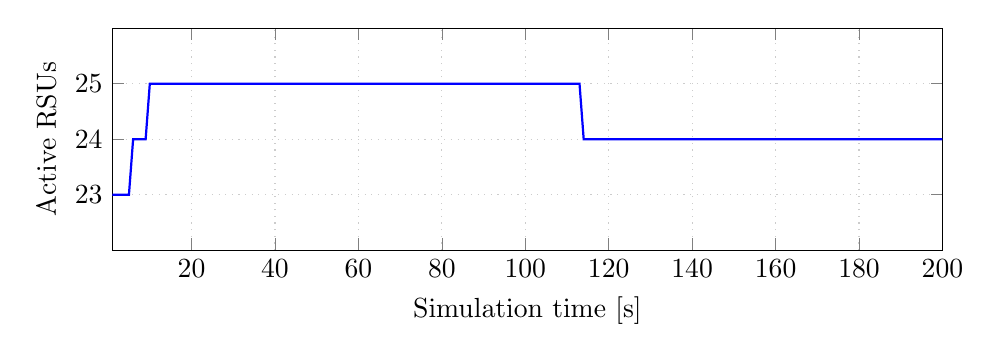
\begin{tikzpicture}
\begin{axis}[
  width=\columnwidth, height=4.4cm,
  ymin=22, ymax=26,
  xmin=1, xmax=200,
  xlabel={Simulation time [s]},
  ylabel={Active RSUs},
  ytick={23,24,25},
  major grid style={dotted,gray!40},
  ymajorgrids=true,
  xmajorgrids=true]
  \addplot+[mark=none, thick] coordinates
   {(1,23)(5,23)(6,24)(9,24)(10,25)(113,25)(114,24)(200,24)};
\end{axis}
\end{tikzpicture}
\caption{NFV lifecycle trace from the full-horizon simulation: two scale-out events raise the active RSU count from 23 to 25, and one scale-in event later reduces it to 24.}
\label{fig:nfv_lifecycle}
\end{figure}

Table~\ref{tab:nfvtelemetry} and Fig.~\ref{fig:nfv_lifecycle} demonstrate that the NFV management plane is highly dynamic. The scenario begins with a baseline of 23 active RSUs (the static junction backbone). As traffic density rises, the orchestrator triggers two separate scale-out events to reach a peak of 25 active edge instances, subsequently executing a scale-in event to reduce the topology to 24 active RSUs as congestion clears. 

These transitions show resource elasticity in the virtualized edge infrastructure. The framework deploys and reclaims RSU functions instead of treating the coverage layer as a fixed, over-provisioned network.

Table~\ref{tab:nfvtelemetry} also reports the application-layer service flows generated by the OMNeT++ control plane. Over the 200\,s horizon, the traffic model maintains up to 4 active emergency vehicles and generates 69 traffic-light preemption requests at signalized junctions.

The control plane also identifies 3 unique simulated collisions. The application logic has both the colliding vehicle and the victim emit an alert, producing 6 \texttt{ACCIDENT\_REPORT} payloads for network-level deduplication handling. Deduplication is deferred to the ns-3 MEC Edge Filter (Use Case 1), which supplies the workload used to exercise broadcast-storm suppression.

All 69 returning preemption commands are executed by the target RSU VNFs. Timing metrics such as traffic-light preemption latency and vehicle braking delay are intentionally omitted from this control-plane summary because they depend on data-plane scheduling and forwarding behavior.

These results indicate that the OMNeT++ NFV layer supplies the orchestration and workload-generation substrate. It decides which RSU edge functions exist, records their lifecycle, and supplies the service events that drive either network stack. NDN then contributes named-data forwarding and caching, while IP contributes the lower-overhead host-addressed baseline.

\subsection{NFV Role in the End-to-End Service Chain}

The NFV component is clearest when the system is read as a service chain rather than as a single protocol experiment. A road event first exists as mobility and application state in SUMO/OMNeT++. The NFV management logic selects the active RSU edge functions, the packet stack carries the resulting messages through IP or NDN, and the OMNeT++ application layer records which service-flow counters were exercised. This keeps lifecycle telemetry, data-plane communication metrics and safety-use-case counters
distinct.

The infrastructure metrics (\code{Active\_RSUs}, \code{Scale\_Out}, \code{Scale\_In}) support claims about dynamic edge coverage; the service-flow metrics (\code{Veh\_Emerg\_Sent}, \code{Veh\_Acc\_Sent}) provide the event counters that the data-plane analysis reacts to.

% =============================================================================
\section{IP/UDP Baseline Results}
\label{sec:ip}
% =============================================================================

The IP/UDP baseline is the lower-overhead host-addressed reference. It does not include NDN PIT, FIB, CS lookup, Interest encoding or Data verification behavior, and it has no in-network cache. The IP table set reports seeds 1--3 for all three numerologies.

\subsection{V2I Latency and Delivery}

Table~\ref{tab:ipqos} reports the three-seed QoS summary. Mean median V2I RTT falls from 8.945\,ms at $\mu=1$ to 4.558\,ms at $\mu=3$. PDR remains close to 99\,\%. 

Table~\ref{tab:ipmu3stats} reports the per-seed values underlying these summaries; the seed-1 anomaly visible in the P99 column recurs in the NDN evaluation and is discussed in Section~\ref{sec:ndn}.

\begin{table}[!t]\centering
\caption{IP/UDP baseline QoS summary over seeds 1--3. Entries report mean and 95\,\% t-interval half-width.}
\label{tab:ipqos}
\scriptsize
\setlength{\tabcolsep}{3pt}
\begin{tabular}{@{}lccc@{}}
\toprule
Metric & \micro$=1$ & \micro$=2$ & \micro$=3$\\
\midrule
V2I avg RTT [ms] & $9.330{\pm}0.398$ & $6.073{\pm}0.252$ & $5.620{\pm}1.247$\\
V2I P50 RTT [ms] & $8.945{\pm}0.224$ & $5.636{\pm}0.117$ & $4.558{\pm}1.039$\\
V2I P95 RTT [ms] & $11.076{\pm}0.654$ & $7.088{\pm}0.643$ & $15.079{\pm}0.371$\\
V2I P99 RTT [ms] & $24.838{\pm}3.993$ & $18.803{\pm}0.359$ & $16.023{\pm}1.203$\\
PDR [\%] & $99.54{\pm}1.92$ & $99.49{\pm}2.14$ & $99.38{\pm}2.55$\\
V2V RTT [ms] & 2.025 & 2.025 & 2.025\\
CS hit rate [\%] & 0.00 & 0.00 & 0.00\\
\bottomrule
\end{tabular}
\end{table}

\begin{table}[!t]\centering
\caption{IP/UDP seed grid for the main V2I latency percentiles. Values are milliseconds.}
\label{tab:ipmu3stats}
\scriptsize
\setlength{\tabcolsep}{3pt}
\begin{tabular}{@{}lrrrrrr@{}}
\toprule
\multirow{2}{*}{\micro} & \multicolumn{3}{c}{P50 RTT} & \multicolumn{3}{c}{P99 RTT}\\
\cmidrule(lr){2-4}\cmidrule(l){5-7}
& s1 & s2 & s3 & s1 & s2 & s3\\
\midrule
1 & 8.850 & 9.029 & 8.957 & 23.671 & 24.171 & 26.671\\
2 & 5.654 & 5.582 & 5.671 & 18.886 & 18.636 & 18.886\\
3 & 5.002 & 4.171 & 4.502 & 15.743 & 15.743 & 16.582\\
\bottomrule
\end{tabular}
\end{table}


\subsection{IP Traffic Counters}

The IP baseline transmitted 666\,965 UDP packets (45.98\,MB) at each numerology, while mean received packet counts ranged from 663\,909 down to 662\,849 across $\mu=1$ to $\mu=3$, a minor variance consistent with the PDR values reported in Table~\ref{tab:ipqos}. The transmitted volume remains perfectly invariant because the offered application load is fixed, whereas the slight drops in received counts occur because the underlying NR numerology and scheduler state affect which replies arrive within the strict measurement window.

Per-flow request/response pairs are recorded for the \code{traffic\_info}, \code{traffic\_count}, \code{safety}, and \code{position\_to\_mec} flows. These underlying metrics support the claim that the IP baseline represents a real request--reply workload rather than a synthetic latency constant. By construction, all NDN forwarding counters are zero within this baseline configuration.

Table~\ref{tab:ipflows} expands the IP baseline by flow. The traffic-info and traffic-count flows show the cleanest monotonic median improvement. The safety and position flows reveal why the aggregate P95 at $\mu=3$ should be interpreted carefully: the typical case improves, but some flows have rare long replies that inflate high percentiles and maxima.

\begin{table*}[!t]\centering
\caption{IP per-flow RTT statistics, seed\,1. Values are milliseconds unless noted.}
\label{tab:ipflows}
\footnotesize
\begin{tabular}{@{}llrrrrrr@{}}
\toprule
Flow & \micro & responses & PDR [\%] & avg & P50 & P95 & P99\\
\midrule
\code{traffic\_info} & 1 & 160,866 & 98.73 & 9.178 & 9.171 & 10.850 & 17.171\\
                     & 2 & 160,525 & 98.52 & 5.864 & 5.779 & 6.975 & 9.654\\
                     & 3 & 159,986 & 98.19 & 5.770 & 5.529 & 6.430 & 6.743\\
\code{traffic\_count}& 1 & 80,271  & 98.78 & 9.186 & 9.207 & 10.814 & 17.171\\
                     & 2 & 80,271  & 98.78 & 5.886 & 5.814 & 6.975 & 9.636\\
                     & 3 & 80,268  & 98.78 & 5.684 & 5.287 & 6.332 & 7.118\\
\code{safety}        & 1 & 320,112 & 98.78 & 9.408 & 8.993 & 10.743 & 30.171\\
                     & 2 & 319,407 & 98.56 & 6.159 & 5.725 & 6.939 & 21.136\\
                     & 3 & 318,761 & 98.36 & 5.913 & 4.529 & 15.252 & 15.868\\
\code{position}      & 1 & 96,727  & 98.00 & 8.238 & 7.279 & 11.243 & 19.671\\
                     & 2 & 96,727  & 98.00 & 5.526 & 4.921 & 6.993 & 17.886\\
                     & 3 & 95,974  & 97.23 & 6.039 & 3.520 & 14.993 & 15.743\\
\bottomrule
\end{tabular}
\end{table*}

\subsection{IP Safety and V2V Scope}

The IP safety block reports 4\,000 checks for each numerology, reflecting the 200\,s horizon and the 50\,ms safety-check interval. Collision warnings and slow-down commands are identical across numerology because they are driven by the same mobility trace and application schedule. V2V latency is exactly 2.025\,ms for all three IP runs, which is expected from the deterministic point-to-point emulation. We therefore use IP V2V values only as a sanity check for the emulated path, not as a radio claim.

% =============================================================================
\section{NDN Co-Simulation Results}
\label{sec:ndn}
% =============================================================================

The NDN dataset contains nine runs: $\mu=1,2,3$ crossed with seeds 1--3. Table~\ref{tab:ndnindexv2} is the master result table.

\begin{table*}[!t]\centering
\caption{NDN master run index and core performance metrics.}
\label{tab:ndnindexv2}
\footnotesize
\begin{tabular}{@{}ccrrrrrrrr@{}}
\toprule
\micro & Seed & V2I Avg & V2I P50 & V2I P95 & V2I P99 & PDR [\%] & ISR [\%] & CS Hit [\%]\\
\midrule
1 & 1 & 19.060 & 15.987 & 48.058 & 58.130 & 97.98 & 99.69 & 55.93\\
1 & 2 & 19.829 & 15.987 & 48.058 & 54.058 & 99.96 & 99.97 & 57.02\\
1 & 3 & 20.498 & 15.987 & 48.130 & 52.557 & 99.96 & 99.97 & 57.02\\
2 & 1 & 12.307 & 10.094 & 36.130 & 43.630 & 97.98 & 99.69 & 55.93\\
2 & 2 & 13.891 & 10.094 & 36.165 & 39.130 & 99.96 & 99.97 & 57.02\\
2 & 3 & 14.105 & 10.094 & 36.165 & 51.165 & 99.96 & 99.97 & 57.02\\
3 & 1 & 12.750 & 7.416 & 30.665 & 34.165 & 97.90 & 99.67 & 55.96\\
3 & 2 & 12.803 & 7.415 & 30.665 & 32.236 & 99.96 & 99.97 & 57.02\\
3 & 3 & 14.032 & 7.416 & 31.683 & 38.165 & 99.96 & 99.97 & 57.01\\
\bottomrule
\end{tabular}
\end{table*}

\subsection{Latency and Numerology}

NDN median V2I latency decreases strongly with numerology: 15.987\,ms at $\mu=1$, 10.094\,ms at $\mu=2$, and approximately 7.416\,ms at $\mu=3$. The $\mu=3$ runs are therefore the only NDN runs that satisfy the P50$\le10$\,ms URLLC-tier flag. All NDN runs remain below the 25\,ms median-level aLM threshold and the 100\,ms general V2X ceiling.

The tail also improves in mean as numerology increases. Averaging the three seeds yields NDN P99 values of approximately 54.92, 44.64 and 34.86\,ms for $\mu=1,2,3$. The study tail analysis shows that the P99 region is associated with retransmission and timeout behavior, with a large share of tail samples carrying one retransmission. This is a more defensible explanation than attributing all tail behavior to CS misses: cache misses, FIB warmup and retransmission dynamics can all contribute, but the measured tail evidence is retransmission-heavy.

Table~\ref{tab:ndnagg} summarizes the NDN seed statistics by numerology. The median is essentially seed-invariant within a numerology, while the tail and PDR are seed-sensitive. This is visible in Table~\ref{tab:ndnindexv2}: seed\,1 is consistently the lower-PDR case, whereas seeds 2 and 3 reach 99.96\,\% PDR. The result suggests that the mobility trace is largely deterministic at the median, but queueing, scheduling and timeout details still affect the tail.

\begin{table*}[!t]\centering
\caption{NDN seed statistics by numerology. Values are mean with 95\,\% t-interval half-width over three seeds.}
\label{tab:ndnagg}
\footnotesize
\begin{tabular}{@{}lrrrrrr@{}}
\toprule
\micro & Avg FullDelay & P50 & P99 & PDR [\%] & CS hit [\%] & ISR [\%]\\
\midrule
1 & 19.796$\pm$1.79 & 15.987$\pm$0.00 & 54.915$\pm$7.16 & 99.30$\pm$2.84 & 56.66$\pm$1.56 & 99.88$\pm$0.40\\
2 & 13.434$\pm$2.44 & 10.094$\pm$0.00 & 44.642$\pm$15.10 & 99.30$\pm$2.84 & 56.66$\pm$1.56 & 99.88$\pm$0.40\\
3 & 13.195$\pm$1.80 & 7.416$\pm$0.00 & 34.855$\pm$7.51 & 99.27$\pm$2.95 & 56.66$\pm$1.51 & 99.87$\pm$0.43\\
\bottomrule
\end{tabular}
\end{table*}

\subsection{Forwarding, Caching and Satisfaction}

The key NDN forwarding metrics remain stable across numerologies: CS hit rate is 55.93--57.02\,\%, ISR is 99.67--99.97\,\%, and no NACKs were observed in all inspected runs. Fig.~\ref{fig:cshr_v2} visualizes this stability. The small seed-1 dip in ISR and PDR appears consistently across numerologies and should be treated as a seed-specific workload/scheduling effect, not as a numerology effect.

The CS hit rate is the most important NDN-specific metric because it shows that the forwarder is not merely tunneling traffic through UDP/IP. The Content Store is actively satisfying repeated requests. The numerology-insensitivity of the hit rate is also meaningful: cache behavior follows the request sequence and freshness policy, whereas latency follows both the request sequence and the radio scheduling granularity.

Table~\ref{tab:ndnfwd_ranges} reports compact forwarding ranges across the nine NDN runs. The spread is small for CS hit rate and ISR, but the timeout counter separates seed\,1 from seeds 2--3. Consequently, the seed effect manifests primarily as a tail-reliability effect rather than a median-latency effect.

\begin{table}[!t]\centering
\caption{NDN forwarding range across all nine runs.}
\label{tab:ndnfwd_ranges}
\footnotesize
\begin{tabular}{@{}lr@{}}
\toprule
Metric & Observed range\\
\midrule
Interests out & 258,257--260,929\\
Data in & 255,597--258,264\\
Satisfied Interests & 818,990--828,401\\
Timed-out Interests & 244--2,704\\
NACKs & 0\\
ISR [\%] & 99.67--99.97\\
CS hits & 349,593--356,531\\
CS hit rate [\%] & 55.93--57.02\\
\bottomrule
\end{tabular}
\end{table}

\begin{figure}[!t]\centering
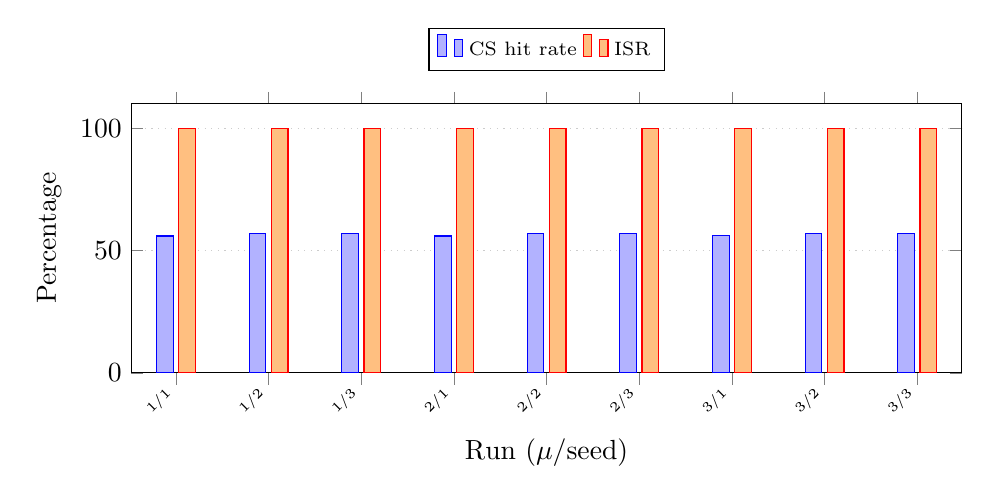
\begin{tikzpicture}
\begin{axis}[
  width=\columnwidth, height=5.0cm,
  ybar=2pt, bar width=6pt,
  ymin=0, ymax=110,
  ylabel={Percentage},
  symbolic x coords={1/1,1/2,1/3,2/1,2/2,2/3,3/1,3/2,3/3},
  xtick=data,
  x tick label style={font=\tiny, rotate=45, anchor=east},
  xlabel={Run ($\mu$/seed)},
  enlarge x limits=0.06,
  legend style={at={(0.5,1.12)},anchor=south, legend columns=2,font=\scriptsize},
  major grid style={dotted,gray!40},
  ymajorgrids=true]
  \addplot+[fill=blue!30] coordinates
   {(1/1,55.93)(1/2,57.02)(1/3,57.02)(2/1,55.93)(2/2,57.02)(2/3,57.02)
    (3/1,55.96)(3/2,57.02)(3/3,57.01)};
  \addplot+[fill=orange!50] coordinates
   {(1/1,99.69)(1/2,99.97)(1/3,99.97)(2/1,99.69)(2/2,99.97)(2/3,99.97)
    (3/1,99.67)(3/2,99.97)(3/3,99.97)};
  \legend{CS hit rate, ISR}
\end{axis}
\end{tikzpicture}
\caption{NDN cache and forwarding behavior across all nine runs. CS hit rate is stable around 56--57\,\%, while ISR remains above 99.67\,\%.}
\label{fig:cshr_v2}
\end{figure}

\subsection{Safety and Internal Use-Case Counters}

NDN accident notification counters are identical across the nine runs: 100 notifications, 8 from RSUs, 92 from MEC, and 0 from cache for the two accident events represented in the evaluated scenario. This does not contradict the overall CS hit rate, because accident notification is a specific UC4 path with its own producer/source distribution. The internal use-case flags show UC1, UC3 and UC4 active in all NDN runs. UC2 traffic-light preemption is true only for $\mu=3$, matching the latency-tier result that only $\mu=3$ provides enough median V2I margin in this scenario.

% =============================================================================
\section{Discussion and Practical Implications}
\label{sec:discussion}
% =============================================================================

\subsection{Latency and Numerology Trade-Offs}

Fig.~\ref{fig:p50p99_v2} compares IP and NDN three-seed means for the main latency percentiles and reveals a clear systems trade-off. IP maintains lower median and $P_{99}$ latency in this dataset due to its lower-overhead, host-addressed communication model, whereas NDN provides architectural capabilities, including in-network caching and name-based forwarding, that are absent from the IP baseline.

\begin{figure}[!t]\centering
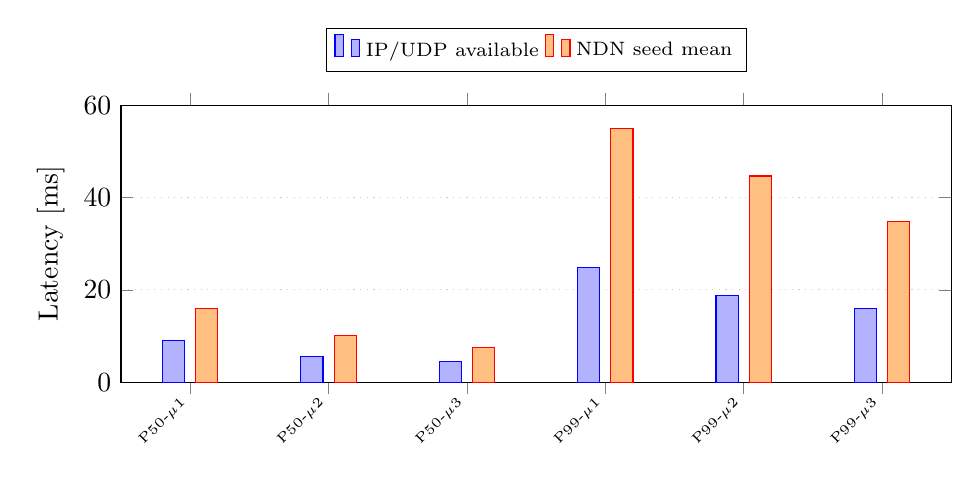
\begin{tikzpicture}
\begin{axis}[
width=\columnwidth,
height=5.1cm,
ybar=4pt,
bar width=8pt,
ymin=0, ymax=60,
ylabel={Latency [ms]},
symbolic x coords={P50-$\mu1$,P50-$\mu2$,P50-$\mu3$,P99-$\mu1$,P99-$\mu2$,P99-$\mu3$},
xtick=data,
x tick label style={font=\tiny, rotate=45, anchor=east},
legend style={at={(0.5,1.12)},anchor=south, legend columns=2,font=\scriptsize},
major grid style={dotted,gray!40},
ymajorgrids=true]
\addplot+[fill=blue!30] coordinates
{(P50-$\mu1$,8.95)(P50-$\mu2$,5.64)(P50-$\mu3$,4.56)
(P99-$\mu1$,24.84)(P99-$\mu2$,18.80)(P99-$\mu3$,16.02)};
\addplot+[fill=orange!50] coordinates
{(P50-$\mu1$,15.99)(P50-$\mu2$,10.09)(P50-$\mu3$,7.42)
(P99-$\mu1$,54.92)(P99-$\mu2$,44.64)(P99-$\mu3$,34.86)};
\legend{IP/UDP available, NDN seed mean}
\end{axis}
\end{tikzpicture}
\caption{V2I latency comparison using three-seed means. The figure is a bounded baseline comparison, not a protocol microbenchmark.}
\label{fig:p50p99_v2}
\end{figure}

The NDN median overhead is approximately 7.0\,ms at $\mu=1$, 4.5\,ms at $\mu=2$, and 2.9\,ms at $\mu=3$ relative to the IP baseline. This overhead is attributable to additional NDN packet processing, name-based forwarding state lookups, and larger wire objects, and decreases as NR slot duration becomes shorter. Consequently, the numerology sweep exposes three operational regimes: at $\mu=1$, the 15.99\,ms median latency exceeds the 10\,ms target and is primarily suitable for cache-oriented studies; at $\mu=2$, the 10.09\,ms median represents a transitional operating point; and at $\mu=3$, the median latency falls to approximately 7.4\,ms while preserving NDN functionality and UC2 support, making it the only evaluated NDN configuration that satisfies the 10\,ms median-latency reference while preserving the evaluated NDN functionality.

High-percentile latency requires more nuanced interpretation. While IP seed-mean $P_{99}$ remains relatively stable between 16--25\,ms, NDN seed-mean $P_{99}$ decreases from approximately 55\,ms at $\mu=1$ to 35\,ms at $\mu=3$. Although CS hits avoid upstream retrieval delays, the tail is dominated by requests that fail to complete on the fast path. Our analysis therefore associates these high percentiles primarily with retransmission and timeout behavior, together with FIB warmup dynamics, indicating that the NDN latency tail reflects the combined effects of radio scheduling constraints and ICN forwarding-state dynamics.

\subsection{Caching and Reliability Advantages}

The principal advantage demonstrated by NDN in this evaluation is not lower raw latency but measurable in-network content reuse. Approximately 56--57\,\% of requests are served as Content Store (CS) hits, a capability structurally absent in the IP baseline. This behavior is particularly valuable for repeated traffic-information and safety-state retrieval, where spatially clustered vehicles request identical content. Furthermore, UC4 demonstrates that topology-aware proactive cache population can integrate naturally with this reuse path. We deliberately do not convert the observed CS hit rate into an equivalent percentage of radio-resource savings, since such a claim would require detailed cache-hit/miss path decomposition and normalized packet-size accounting beyond the scope of this work.

Packet delivery remains high across both stacks, ranging from 98.20--98.65\,\% for IP and 97.90--99.96\,\% for NDN. NDN Interest Satisfaction Rate (ISR) remains above 99.67\,\%, with no NACKs observed in the inspected traces. Throughput is not treated as a direct comparative metric because IP reports per-flow byte-rate summaries whereas NDN reports rate-trace aggregates. Nevertheless, the results indicate that both stacks sustain the configured application workload successfully.

\subsection{Architectural and Deployment Implications}

The inclusion of the NFV orchestration layer provides important context for interpreting the protocol comparison. The evaluated protocols do not operate over an abstract, static service endpoint but over a dynamic edge layout supplied by the OMNeT++ MANO entity. NFV does not inherently reduce NDN latency below the IP baseline; rather, it provides the elastic edge substrate that enables a realistic evaluation of both protocol stacks within a modern 5G architecture.

Taken together, the measured trade-offs suggest that deployment decisions should be driven by application workload rather than protocol preference alone. Latency-sensitive, host-addressed traffic requiring minimal V2I delay favors the simpler IP/UDP baseline, which delivers a $P_{50}$ RTT of approximately 4.5--8.9\,ms with minimal protocol overhead. Conversely, applications characterized by repeated, location-scoped information retrieval justify an NDN deployment when the benefits of approximately 56--57\,\% CS hit rates and native Interest-satisfaction telemetry outweigh the modest median latency penalty, particularly under the $\mu=3$ operating point.

% =============================================================================
\section{Threats to Validity and Limitations}
\label{sec:limits}
% =============================================================================

The experiments characterize how information-centric forwarding behaves when coupled with NFV-managed edge services and NR-V2X mobility conditions, within the constraints defined by the simulation scope described below.

\textit{Seed count and pairing.} The evaluation covers all nine numerology--seed combinations for both stacks. While this supports a controlled cross-stack comparison, it does not constitute an exhaustive statistical campaign across variable topologies. This study therefore emphasizes specific effect sizes and confidence intervals rather than universal protocol rankings.

\textit{Different latency observables.} IP RTT and ndnSIM FullDelay are both application-level latency observables, but they are not identical instrumentation points; the KPI map defines the distinction used in the results.

\textit{V2V is not PC5.} The implementation code explicitly configures V2V as point-to-point emulation, not 3GPP PC5 sidelink. This is because the ns-3/NR architecture used in this study did not provide an integration-ready PC5 sidelink module that could be integrated into the current ns-3/ndnSIM--OMNeT++/Veins co-simulation. V2V latency values therefore describe controlled application/protocol behavior under ideal connectivity. They must not be cited as PC5 Mode 1/2 resource-selection, fading, or contention results.

\textit{Single-gNB V2I topology.} The scenario uses one gNB and reports no handover events. This isolates stack behavior, but it does not exercise producer mobility, FIB updates during handover, multi-cell interference, or MEC relocation.

\textit{Channel and mobility scope.} The channel is UMa-LoS at 3.5\,GHz with 100\,MHz bandwidth. NLoS blockage, dense urban canyon effects, pedestrians and cyclists are outside the dataset. The trace has about 35 vehicles and a 200\,s horizon, which is enough to observe stable cache behavior but not enough to study long-term cache eviction.

\textit{Safety counters are simulation counters.} Collision warnings, emergency brakes, slow-down commands and ``near misses prevented'' are algorithm and simulator counters. They verify that the safety logic ran and produced actions under the trace; they do not prove physical-world crash-prevention performance.

\textit{NFV telemetry scope.} The NFV logs are OMNeT++ management-plane telemetry. They confirm RSU lifecycle activity and accident service-flow counters, but the available service-flow traces do not contain non-zero emergency-vehicle or traffic-light latency samples. Therefore, we do not infer emergency preemption delay from the NFV telemetry.

\textit{Cache interpretation and proactive attribution.} The CS hit rate is a strong NDN-specific signal (consistently exceeding 55\,\%), but it is not automatically equal to the same percentage of end-to-end byte savings.

Furthermore, the current simulation counters aggregate all CS hits globally, precluding the isolation of standard reactive caching from MANO-driven proactive injections.

% =============================================================================
\section{Conclusion and Future Work}
\label{sec:conclusion}
% =============================================================================

This manuscript reports a reproducible NFV-orchestrated V2X-NDN-5G co-simulation study with an IP/UDP baseline and a nine-run NDN dataset. The results demonstrate a quantified trade-off: while IP provides lower median latency, NDN adds stable in-network caching and high Interest satisfaction. In the measured V2I latency distribution, IP has lower median RTT: 8.945, 5.636 and 4.558\,ms as three-seed means for $\mu=1,2,3$. NDN medians are 15.987, 10.094 and about 7.416\,ms. NFV provides the managed edge-service substrate, while NDN adds latency overhead but provides stable in-network caching, high Interest satisfaction, and name-based dissemination semantics that IP does not natively support.

For the present scenario, NDN at $\mu=3$ is the only NDN configuration that meets the evaluated 10\,ms median-latency reference derived from TS\,22.186, though all evaluated NDN runs remain within broader V2X latency bounds. The primary contribution of this study is the empirical, system-level measurement of NFV RSU lifecycle behavior, NDN-over-cellular dynamics, and safety-use-case counters within a unified, reproducible pipeline.

Building upon these findings and acknowledging the structural boundaries of the current simulation scope, several high-priority research directions emerge. Future experiments should prioritize: (1) expanding the seed count, vehicle density range, and map diversity to construct broader cross-stack confidence intervals; (2) replacing V2V point-to-point emulation with a 3GPP NR-V2X PC5 sidelink model to accurately capture radio resource contention; (3) stressing the NFV layer with higher traffic densities and non-zero emergency-preemption events to extract strict traffic-light service latency; (4) introducing multi-gNB handovers and producer-mobility to evaluate FIB continuity and cache utility under topology changes; and (5) evaluating geo-scoped naming schemes and forwarding strategies specifically optimized for vehicular hazard notification.

% =============================================================================
\appendices
\section{Reproducibility}
\label{app:repro}
The simulation is parameterized by duration (200\,s), numerology ($\mu\in\{1,2,3\}$), and seed index (1--3). A 2\,s warm-up period is excluded from all metric calculations. V2V links are modeled as point-to-point emulated connections. All simulation source code, configuration scripts, and generated data are available upon request.
% TODO : Replace last sentence above with:
% All simulation source code, configuration scripts, and extracted datasets are open-source and publicly available at [Insert GitHub/Zenodo Link/DOI here].

\section{Symbols and Acronyms}
\label{abbrev}
To assist the reader, Table~\ref{tab:symbols} summarizes the key acronyms and parameters used throughout this study.

\begin{table}[!htbp]\centering
\caption{Symbols and Abbreviations}
\label{tab:symbols}
\footnotesize
\begin{tabular}{@{}p{0.22\linewidth}p{0.70\linewidth}@{}}
\toprule
Symbol/Acronym & Meaning\\
\midrule
$\mu$ & NR numerology; subcarrier spacing $15\cdot2^\mu$\,kHz\\
CS & NDN Content Store\\
FIB & Forwarding Information Base\\
ISR & Interest Satisfaction Ratio\\
MEC & Multi-access Edge Computing\\
NFV & Network Functions Virtualization\\
MANO & Management and orchestration\\
PDR & Packet Delivery Ratio\\
PIT & Pending Interest Table\\
RTT & Round-trip time\\
TTC & Time-to-Collision\\
V2I & Vehicle-to-Infrastructure\\
V2V & Vehicle-to-Vehicle\\
\bottomrule
\end{tabular}
\end{table}

% =============================================================================
\section*{Acknowledgment}
% %please keep this acknowledgement section. -- BRD.
This research was partly supported by Tribhuvan University Research Directorate under National Priority Area Research with Grant ID: TU-NPAR-081/82-MRG-01 principally investigated by Dr. Babu R. Dawadi


\begin{thebibliography}{99}
\bibitem{ref:v2x-3gpp22186}
3GPP TS\,22.186, ``Service requirements for enhanced V2X scenarios,''
3rd Generation Partnership Project, Tech.\ Spec.\ V17.0.0, 2022.
\bibitem{ref:v2x-3gpp22886}
3GPP TR\,22.886, ``Study on enhancement of 3GPP support for 5G V2X
services,'' 3rd Generation Partnership Project, Tech.\ Rep., 2018.
\bibitem{ref:v2x-3gpp22185}
3GPP TS\,22.185, ``Service requirements for V2X services,''
3rd Generation Partnership Project, Tech.\ Spec.\ V17.0.0, 2022.
\bibitem{ref:nr-phy}
3GPP TS\,38.211, ``NR; Physical channels and modulation,''
3rd Generation Partnership Project, Tech.\ Spec., Rel.\ 17, 2022.
\bibitem{ref:nr-channel}
3GPP TR\,38.901, ``Study on channel model for frequencies from 0.5 to
100 GHz,'' 3rd Generation Partnership Project, Tech.\ Rep., 2020.
\bibitem{ref:ndn-overview}
L.~Zhang, A.~Afanasyev, J.~Burke \emph{et al.}, ``Named data networking,''
\emph{ACM SIGCOMM Computer Communication Review}, vol.~44, no.~3,
pp.~66--73, 2014.
\bibitem{ref:nfd}
A.~Afanasyev \emph{et al.},
``NFD developer's guide,''
NDN Team, Technical Report NDN-0021, Revision 10, 2018.
\bibitem{ref:vndn}
G.~Grassi \emph{et al.}, ``VANET via named data networking,'' in
\emph{Proc. IEEE INFOCOM Workshops}, 2014.
\bibitem{ref:ndn-v2x-survey}
M.~Amadeo, C.~Campolo, and A.~Molinaro,
``Information-centric networking for connected vehicles: A survey and future perspectives,''
\emph{IEEE Communications Magazine},
vol.~54, no.~2, pp.~98--104, 2016.
\bibitem{ref:ndnsim}
S.~Mastorakis, A.~Afanasyev, and L.~Zhang, ``On the evolution of ndnSIM: 
an open-source simulator for NDN experimentation,'' 
\emph{ACM SIGCOMM Computer Communication Review}, vol.~47, no.~3, 
pp.~19--33, 2017.
\bibitem{ref:ns3-nr}
N.~Patriciello \emph{et al.}, ``An E2E simulator for 5G NR networks,'' 
\emph{Simulation Modelling Practice and Theory}, vol.~96, p.~101933, 2019.
\bibitem{ref:sumo}
P.~A.~Lopez \emph{et al.}, ``Microscopic traffic simulation using
SUMO,'' in \emph{2018 21st International Conference on Intelligent
Transportation Systems (ITSC)}, 2018, pp.~2575--2582.
\bibitem{ref:veins}
C.~Sommer, R.~German, and F.~Dressler,
``Bidirectionally coupled network and road traffic simulation
for improved IVC analysis,'' \emph{IEEE Transactions on Mobile
Computing}, vol.~10, no.~1, pp.~3--15, 2011.
\bibitem{ref:mec-etsi}
ETSI GS MEC 003, ``Multi-access edge computing; framework and reference
architecture,'' ETSI Group Spec., 2020.
\bibitem{ref:ttc}
M.~Minderhoud and P.~Bovy, ``Extended time-to-collision measures for road 
traffic safety assessment,'' \emph{Accident Analysis \& Prevention}, 
vol.~33, no.~1, pp.~89--96, 2001.
\bibitem{ref:ndn-mobility}
B.~Feng, H.~Zhou, and Q.~Xu,
``Mobility support in named data networking: a survey,''
\emph{EURASIP Journal on Wireless Communications and Networking},
vol.~2016, no.~1, p.~220, 2016.
\bibitem{ref:ndn-cache-survey}
A.~Ioannou and S.~Weber,
``A Survey of caching policies and forwarding mechanisms in information-centric networking,''
\emph{IEEE Communications Surveys \& Tutorials},
vol.~18, no.~4, pp.~2847--2886, 2016.
\bibitem{ref:cv2x-rel16}
3GPP TR\,38.886, ``V2X Services based on NR; User equipment (UE)
radio transmission and reception,'' 3rd Generation Partnership
Project, Tech.\ Rep., Rel.\ 16, 2020.
\bibitem{ref:idm}
M.~Treiber, A.~Hennecke, and D.~Helbing,
``Congested traffic states in empirical observations and microscopic simulations,''
\emph{Physical Review E},
vol.~62, no.~2, pp.~1805--1824, 2000.
\bibitem{ref:mobil}
A.~Kesting, M.~Treiber, and D.~Helbing,
``General lane-changing model MOBIL for car-following models,''
\emph{Transportation Research Record},
vol.~1999, no.~1, pp.~86--94, 2007.
\bibitem{ref:5g-urllc}
H.~Ji, S.~Park, J.~Yeo, Y.~Kim, J.~Lee, and B.~Shim, 
``Ultra-reliable and low-latency communications in 5G downlink: 
Physical layer aspects,'' \emph{IEEE Wireless Communications}, 
vol.~25, no.~3, pp.~124--130, 2018.
\bibitem{ref:mec-v2x-placement}
A.~Moubayed, A.~Shami, P.~Heidari, A.~Larabi, and R.~Brunner,
``Edge-enabled V2X service placement for intelligent transportation systems,''
\emph{IEEE Transactions on Mobile Computing},
vol.~20, no.~4, pp.~1380--1392, 2021.
\end{thebibliography}

\end{document}
